\documentclass[11pt, twocolumn]{article}
\usepackage[utf8]{inputenc}
\usepackage{cite}
\usepackage{url}
\usepackage{multicol}
\usepackage[letterpaper, margin=0.75in]{geometry}
\usepackage{enumitem}
\setlength{\columnsep}{0.5in}
\usepackage{graphicx}
\usepackage{tabto}
\usepackage{array,url,kantlipsum}
\usepackage{float}

\begin{document}
\twocolumn[{%
 \vspace*{25px}
 \centering
 \LARGE Six Degrees of Collaboration \\ A Predator Pack's Guide to Success \\[1.5em]
 \large Sami Ghoche,
        George Lok,
        Devvret Rishi\\[1em]
        
CS289 Final Project\\
Harvard University
  \vspace*{50px}
}]

\begin{abstract}

We introduce different collaboration policies for a pack of predators chasing a moving prey, ranging from complete collaboration to no collaboration at all. We operate in two settings: In the first setting, all predators can observe each other and their prey at all times, whereas in the second setting, predators can only observe what is directly in their line of sight. In the first setting, we present six collaboration policies that vary in efficiency both in terms of computational complexity and rate of success. In addition to evaluating the tradeoffs between these six mechanisms, we also present a successful trapping heuristic for a pack of coordinating predators. In the second setting, we present and compare two alternative search and destroy strategies through stigmergic communication. Our contributions will be useful for studies of predator/prey models in general, but may specifically be applicable in law enforcement settings involving a team of police officers chasing a fugitive from justice. 

\end{abstract}

\section{Introduction}
In nature, we observe that predator animals (including human beings) often collaborate when chasing a prey. This is because in some settings, a team of collaborating predators can achieve outcomes that separated individuals cannot, such as outcomes resulting from trapping behavior. However, collaboration nearly always exhibits large costs. First, collaborating agents have to split their rewards with their collaborators. In the animal world, this means gaining fewer resources; in law enforcement, this may mean receiving less credit for capturing criminals. Furthermore, collaboration always requires a form of coordination, and coordination is expensive. For example, we can consider "perfect collaboration", whereby many predator agents act as a single unit that makes a single decision involving the movement of every agent in the team. This is essentially the same as having a centralized controller or a brain that directs each agent in the team. Such a centralized system though is not scalable, and there has been much research directed at developing scalable multi-agent systems in which computation is distributed among agents. In this paper, we assume that predators consider each other as collaborators instead of competitors, and they strive jointly to maximize an aggregate reward, meaning that all agents benefit equally when the prey is captured, regardless of which predator captured it. We also disregard the free-rider problem and assume that all predators actively make an effort to help the team instead of relying on other collaborators and reaping the benefits of the capture. For our experiments, we used the Berkeley Pacman framework \cite{Pacman}. because it allows for very general predator/prey model simulations. We operate in two settings: In the first setting, all predators can observe each other and their prey at all times, whereas in the second setting, predators can only observe what is directly in their line of sight. In the first setting, we present six different collaboration strategies with varying degrees of collaborative cost and efficiency: 1- Fully centralized collaboration. 2- Fully centralized collaboration of loosely coupled subteams. 3- Encrypted communication of actions between predators. 4- Communication of actions between predators that can be overheard by a prey. 5- Individual actions while taking into account positions of other predators. 6- No collaboration at all. The first five of these strategies require the notion of trapping behavior, and one of the main contributions of this paper is a successful heuristic that leads to trapping behavior. In the second setting, agents leave stigmergic trails behind them that decay with time, this is reminiscent of many examples of stigmergic communication observed in nature (for example in foraging ants [REFERENCE]). We compare two alternative strategies that predators can use to interact with the stigmergic trails that others leave behind. 1- Avoid these trails in an attempt to split up effectively and capture the prey. 2- Follow these trails in an attempt to congregate and corner the prey when it is found.\\
\indent The paper is organized into the following sections: Section 2 describes related work. Section 3 provides detailed descriptions with theoretical considerations of our six strategies in the first setting, and two strategies in the second setting. Section 4 describes our implementation using the Berkeley Pacman framework and the experiments we conducted. Section 5 presents our results and discusses them. Section 6 states our conclusions and future directions. 

\section{Related Work}

 
\section{Description of Proposed Strategies}
\subsection{First Setting}
In the first setting, we propose six different strategies. Here they are in decreasing order of computational complexity:\\
\begin{enumerate}[leftmargin=0.25cm]
	\item Fully centralized collaboration\\
	In this strategy, we treat the predators as a single unit (called a team). Thus, a team's action is called a joint action. Joint action $\vec{a} = <a_1, a_2, ..., a_n>$, where $N$ is the number of predators. A centralized controller will evaluate every possible joint action, and select the joint action with the highest value. If there are at most $M$ possible actions a predator can take at any time step $t$, and a total of $T$ time-steps, the computational complexity of this strategy in every time-step will be $O(M^N)$ and thus, for the entire duration of the pursuit, the complexity would be $O(TM^N)$.
	
	\item Fully centralized collaboration of loosely coupled subteams\\
	In this strategy, we split the predators into $K$ subteams as evenly as possible. Each subteam $k$ will have a joint action $\vec{a_k}$. Joint action $\vec{a_k} = <a_1, a_2, ..., a_{\frac{N}{K}}>$. There is a centralized controller for each subteam that evaluates every possible joint action for that subteam and selects the one with the highest value. Since the computation for each subteam can be run in parallel, the complexity for this algorithm in one time-step will be $O(M^{\frac{N}{K}})$, and for the entire duration of the pursuit, the complexity would be $O(TM^{\frac{N}{K}})$. Therefore, this algorithm is asymptotically much faster than the first one, but its speed comes at a cost, since optimal joint actions for subteams might result in suboptimal joint actions for the larger team as a whole. 
	
	\item Encrypted communication of actions between predators.\\
	In this strategy, each predator decides which action to take on its own, but it takes into account the positions of other predators. This is important because predators will try to avoid each other in an attempt to minimize the area that the prey can maneuver in, effectively trapping it. However, since predators take individual decisions, they don't have a model of other predator's behaviors so they only take into account the current positions of other predators not where they are going to be in the next time step, which results in suboptimal decision-making based on inaccurate information. Communication can help with this problem: we can have predators take turns in deciding on an action and communicating it to all other predators once they have committed to it. So for example, predator 1 will decide on action $a_1$, and communicate it to predator 2, who will decide on $a_2$ based on the current positions of all other predators while taking into account predator 1's position AFTER taking action $a_1$. Predator 2 then communicates $a_2$ to predator 3, who decides on an action based on the positions of other predators and the positions that predators 1 and 2 will be in after taking actions $a_1$ and $a_2$ respectively, etc. until the last predator has a full picture of where all other predators will be and makes its decision based on those accurate future positions. Furthermore, we assume that communication is encrypted so the prey cannot overhear the communication and use it to its advantage. Each predator will look at the positions of each of the $N-1$ others and then evaluate each of the $M$ actions available to it. Since the predators have to wait for each other in turn, each time step will have a computational complexity of $O(N(N+M))$. Thus, the entire pursuit will have a complexity of $O(TN(N+M))$. This is exponentially faster than the first two algorithms, but the joint actions that this strategy yields in the end may be suboptimal. Additionally, there is a logistic cost to being able to communicate that we call $C$. This cost varies depending on the predator/prey domain. For example, in a law enforcement setting, this can be the cost of purchasing and maintaining walkie talkies. Since messages are securely encrypted in this strategy, there's another additional logistic cost that we call $S$. 
	
	\item Communication of actions between predators that can be overheard by the prey\\
	This strategy is very similar to the third one, except that at each step, the prey can overhear the entire communication between the predators because communication is not encrypted. This added information should allow the prey to take decisions faster (since it does not have to evaluate all possible actions of predators) and it will also reduce the uncertainty that the prey deals with and allow it to take decisions based on a more accurate belief model. As above, each time step will have a computational complexity of $O(N(N+M))$. Thus, the entire pursuit will have a complexity of $O(TN(N+M))$. Similarly, we still incur a logistic cost of $C$ because we are communicating, but there is no additional cost $S$ because the communication is no longer secure. 
	
	\item Individual actions while taking into account positions of other predators\\
	This strategy is similar to the previous two. However, there is no communication between predators here, so predators independently look at each other's current positions and take actions based on these current positions. Since predators no longer have to wait for each other in order to take decisions, the computation can be parallelized among the predators. So each time step will have a computational complexity of $O(N+M)$ and the entire pursuit will have a complexity of $O(T(N+M))$. This is linearly faster than the previous two algorithms and does not incur communication costs but actions are taken individually based on inaccurate information and are thus less optimal than in the previous two algorithms. 
	
	\item No collaboration at all
	In this strategy, predators do not collaborate or coordinate in any way. They simply each independently decide to chase the prey and take the action that minimizes their distance to the prey's current position. Assuming that distance evaluation takes constant time, we can parallelize the computation among the predators and conclude that the computational complexity of one time step is $O(M)$ and the computational complexity of the entire pursuit is $O(TM)$. It is important to note that while this strategy is by far the least complex, it does not inherently lead to any trapping behavior and essentially only allows for capturing the prey through accidental trapping (since we assume that the predators and the prey have the same speed and that the prey actively tries to evade predators).  
\end{enumerate}

\subsection{Second Setting}
In the second setting, we propose two different strategies revolving around the use of stigmergy.  The basic principle is that ghosts leave trails that other ghosts can see. The amount of trail left can depend on when ghosts see Pacman.  Ghosts will with high probability chase after Pacman if they see them.  Ghosts keep track of Pacman's last known position, and are biased to go towards that position if they don't see Pacman.  This last known position is reset if they arrive at the position and do not see Pacman.

\begin{enumerate}[leftmargin=0.25cm]
	\item Attractive Stigmergy\\
 	In attractive stigmergy, ghosts do not lay trails unless they either see Pacman or have an idea where Pacman is.  They lay more trail if they see Pacman than if they only have an idea where Pacman is.  Ghosts are more likely to choose a path that has more trail on it.  Finally, to prevent backtracking and to prevent them from sticking together, ghosts explicitly are less likely to take the reverse direction of the last action they do and are less likely to make an action that puts them on top of another ghost.
	
	\item Repulsive Stigmergy\\
	Taking advantage of the fact that we only need one ghost to capture Pacman, ghosts always lay trail, but lay significantly more trail if they see Pacman.  Ghost are more likely to choose a path that has less trail on it.  There's no need to prevent backtracking explicitly since the ghosts are unlikely to backtrack on their own trail.
\end{enumerate}

// INSERT DIAGRAMS HERE WITH FLOWCHART OF STIGMERGY ALGORITHMS


\section{Experimental Setup}
\subsection{General}
We simulated our approaches for both settings on the Berkeley Pacman game platform because it lent itself well to the general pattern of predator/prey models and was flexible enough to allow all the behavior that we wanted to simulate. In the Pacman game, the prey is a Pacman agent, and the predators are one or many ghosts. In the original game, Pacman moves around a map collecting food, and he wins once all the food on the map has been collected. He loses when a ghost catches him. For our purposes, we eliminated the notion of food and winning, we kept the penalty associated with being caught, and we gave Pacman a reward for surviving each time step, thus incentivizing survival. Here is an example of what the game looks like: \\\\
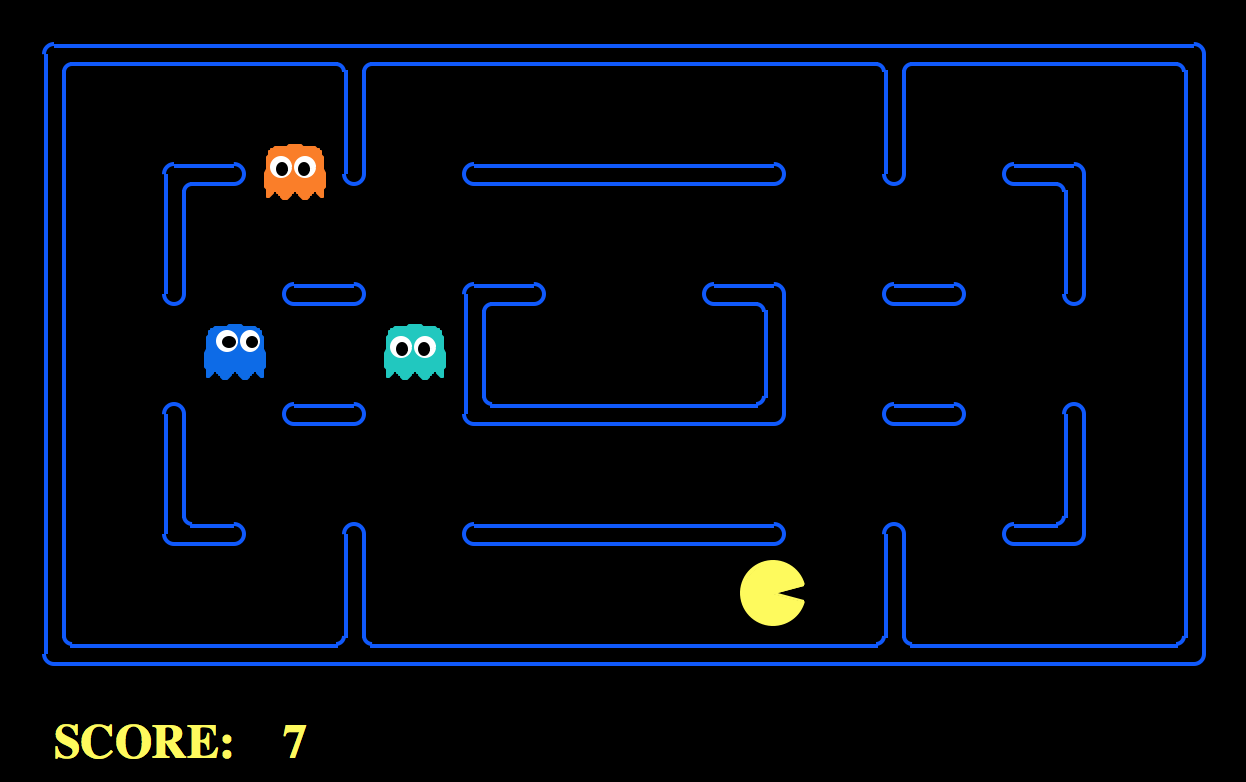
\includegraphics[scale=0.4]{examplemap.png}\\\\
When we load in a map, we first convert it into a graph where each position (x, y coordinate) is only connected to positions that are reachable from it in one step (agents cannot go through walls). Once we have our graph, we precompute the shortest distances between any two positions in the map, using Floyd Warshall's cubic-runtime algorithm. These distances are stored and accessed in constant time by all agents at every step of the game. For example, in strategy 6, we simply make each ghost pick whatever action minimizes its distance to Pacman. For all of the other strategies, ghosts take distance into consideration, but there is also the added notion of trapping Pacman. We came up with a heuristic that successfully encourages ghosts to reduce the area that Pacman can maneuver in. Note that we introduce a bit of randomness in all algorithms just to account for different scenarios and generate more realistic simulations.\\
\subsection{Pacman Behavior}
It's important here to mention how Pacman behaves. We modeled Pacman as a Minimax Alpha-Beta pruning agent. At depth $d$, Pacman evaluates a particular state $s$ by the distance to the ghost closest to it. So Pacman tries to maximize this distance, while it assumes that ghosts actively try to minimize it. This is an accurate vision of the world but it is however lacking the knowledge that ghosts will try to trap it. This is because of two reasons. First, ghosts may not always be trying to trap Pacman (strategy 6 for example). Second, it's not realistic to assume that Pacman has a complete mental model of the other ghosts and is able to simulate the computations of all other ghosts before taking its action.\\
One more thing we should mention about Pacman is that in the case of strategy 4 in which Pacman overhears ghosts' communication, Pacman basically gains a depth of minimax for free because it knows exactly where the ghosts will be in one step. More importantly, Pacman's decision in this case is based on a more accurate model of the world, since Pacman no longer has to maximize a heuristic that does not take trapping into account, it can know exactly what the ghosts will do in the first step.

\subsection{First Setting}
\subsubsection{Trapping Heuristic}

\begin{figure}
	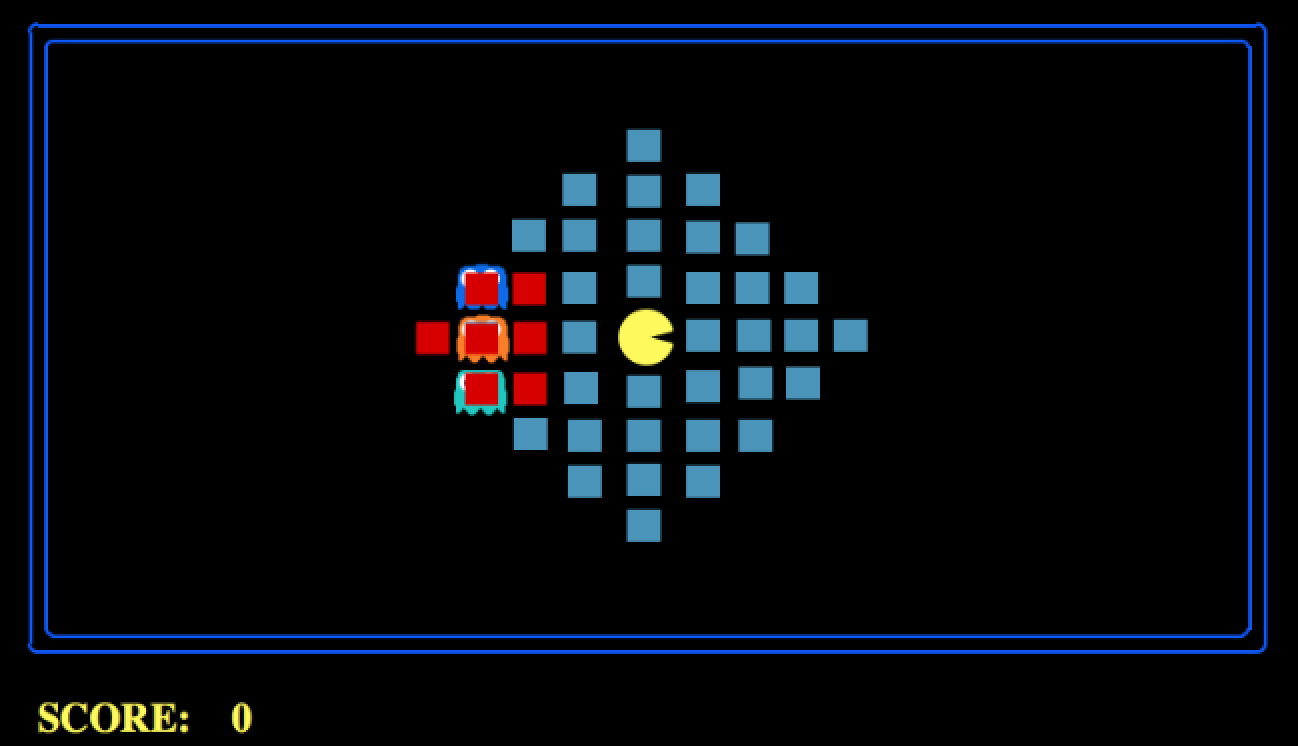
\includegraphics[width=\columnwidth]{badheuristic.png}
	\caption{Bad Heuristic}
	\label{fig:badheuristic}
\end{figure}

\begin{figure}
	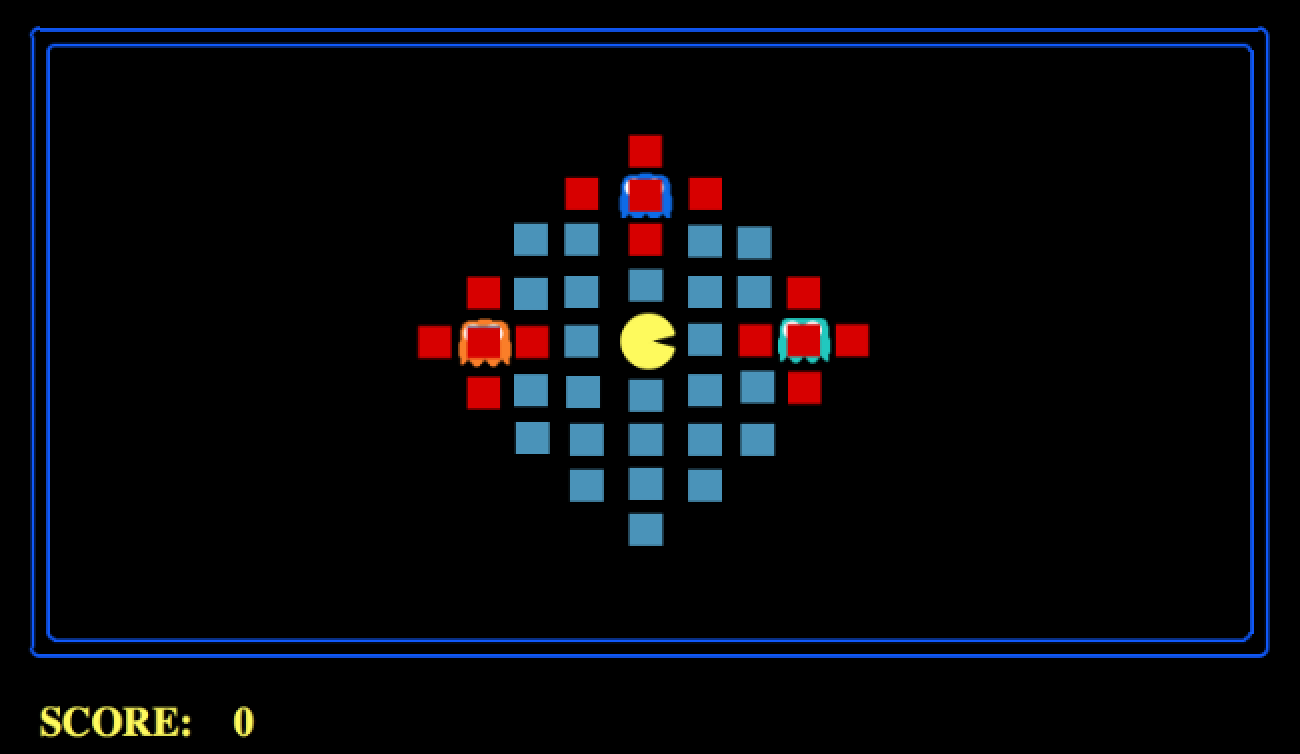
\includegraphics[width=\columnwidth]{goodheuristic.png}
	\caption{Good Heuristic}
	\label{fig:goodheuristic}
\end{figure}

This heuristic consists of two features. The first feature pertains to the distance between the ghost and Pacman. The second heuristic can be described as the total number of positions that are unsafe for pacman to be in, within a radius $r$. A position is unsafe if a ghost needs only one action to get there. To illustrate this, we can look at the following two images where the blue dots represent all the safe positions for Pacman within radius 4 and the red dots represent all the unsafe positions within radius 4. In figure \ref{fig:badheuristic}, the ghosts are close to each other so they only make seven dots unsafe. In figure \ref{fig:goodheuristic}, the ghosts are trapping pacman and they make 15 dots unsafe.\\ 

In the end, we settled on the following heuristic for each state $s$:
$$h(s) = u - 1.5d$$ Where $u$ is the number of unsafe positions in state $s$ within radius $r$, and $d$ is the distance to Pacman. This heuristic incentivizes both getting closer to Pacman (in order to minimize the distance and get within the radius $r$), as well as getting further away from each other.

\begin{figure}
	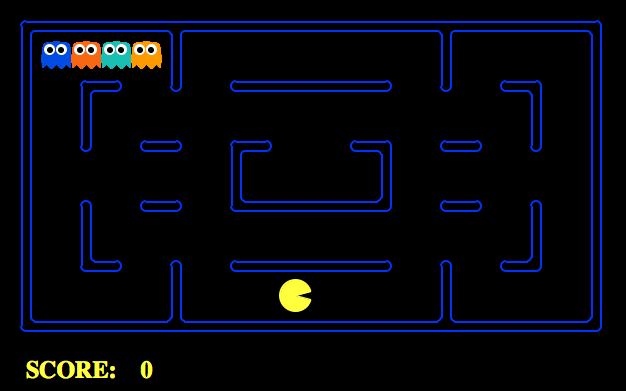
\includegraphics[width=\columnwidth]{maptogether.png}\\
	\caption{Map Together}
	\label{fig:maptogether}
\end{figure}

\begin{figure}
	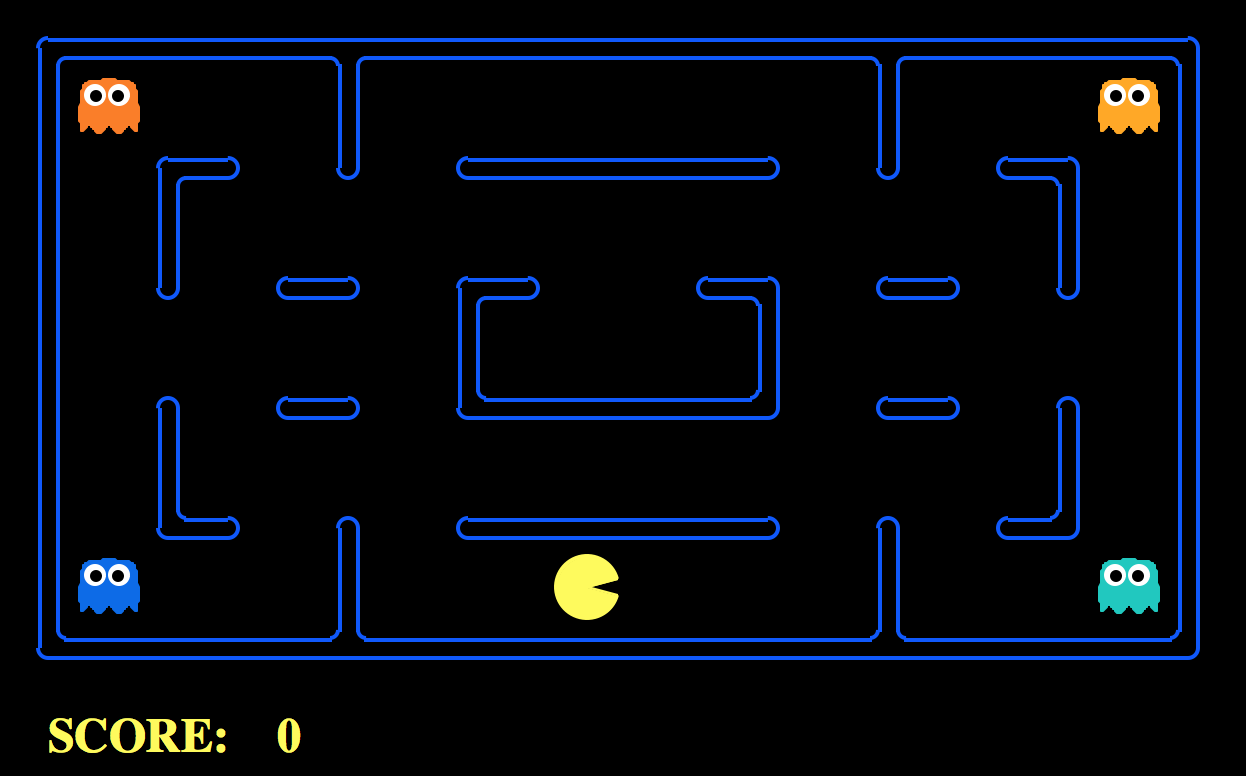
\includegraphics[width=\columnwidth]{mapcorners.png}\\
	\caption{Map Corners}
	\label{fig:mapcorners}
\end{figure}

\subsubsection{Experiments}
We ran each algorithm for 100 games with 2, 3 and 4 ghost agents for each of two initial configurations. In the first initial configuration, all ghosts started off very close to each other in the top left corner of the map. In the second initial configuration, ghosts started off each at a corner of the map. The initial configurations are shown below for 4 ghosts:\\\\


\subsection{Second Setting}

\pagebreak

\section{Results and Discussion}

Now we will discuss our results from running the simulations described in experimental setup. 

%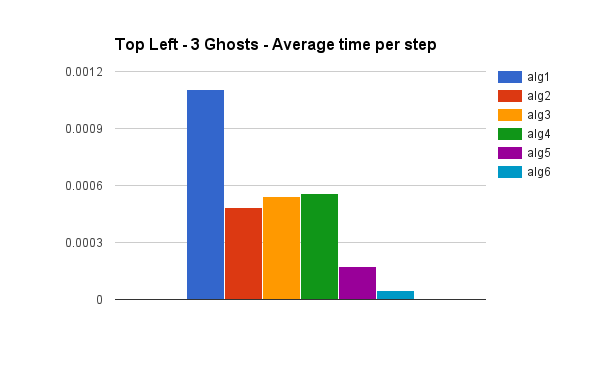
\includegraphics[width=\columnwidth]{time.png}

\begin{figure}[H]
	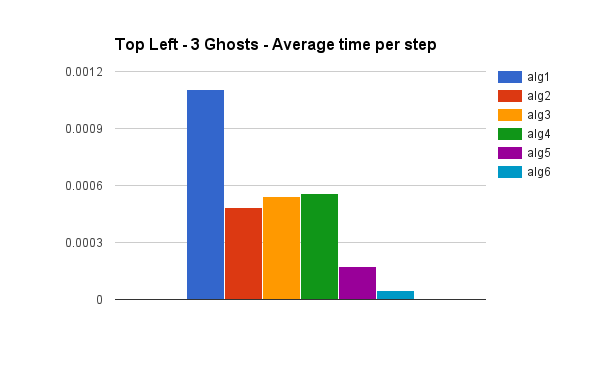
\includegraphics[width=\columnwidth]{time.png}
	\caption{Average Computation Time Per Step}
	\label{fig:averagecomputation}
\end{figure}	

Some words about the previous figure. 

\begin{figure}[H]
	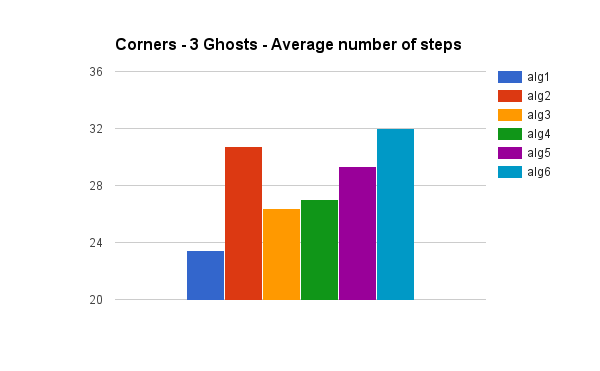
\includegraphics[width=\columnwidth]{cornersteps.png}
	\caption{Average Number of Steps}
	\label{fig:averagenumsteps}
\end{figure}

adsfasdfsadf

\begin{figure*}[t]
	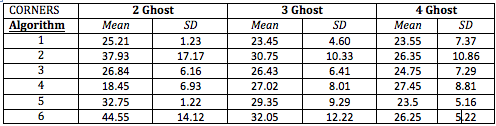
\includegraphics[width=\textwidth]{CornersScore.png}
	\caption{Corner Steps}
	
\end{figure*}

Some words about the other previous figure. 

%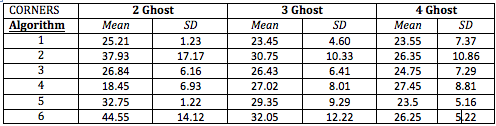
\includegraphics[width=\columnwidth]{CornersScore.png}





\section{Conclusion and Future Directions}

\section{Division of Work}

\section{References}
\bibliographystyle{plain}
\bibliography{bibliography.bib}


\end{document}
